%
% File acl2015.tex
%
% Contact: car@ir.hit.edu.cn, gdzhou@suda.edu.cn
%%
%% Based on the style files for ACL-2014, which were, in turn,
%% Based on the style files for ACL-2013, which were, in turn,
%% Based on the style files for ACL-2012, which were, in turn,
%% based on the style files for ACL-2011, which were, in turn, 
%% based on the style files for ACL-2010, which were, in turn, 
%% based on the style files for ACL-IJCNLP-2009, which were, in turn,
%% based on the style files for EACL-2009 and IJCNLP-2008...

%% Based on the style files for EACL 2006 by 
%%e.agirre@ehu.es or Sergi.Balari@uab.es
%% and that of ACL 08 by Joakim Nivre and Noah Smith

\documentclass[11pt]{article}
\usepackage{acl2015}
\usepackage{times}
\usepackage{url}
\usepackage{latexsym}
\usepackage{graphicx}

%\setlength\titlebox{5cm}

% You can expand the titlebox if you need extra space
% to show all the authors. Please do not make the titlebox
% smaller than 5cm (the original size); we will check this
% in the camera-ready version and ask you to change it back.


\title{WIZARD:Program Synthesis from Natural Pseudocode}

\author{Yu Feng \\
  UT Austin \\
  {\tt yufeng@cs.utexas.edu} \\\And
  Jianyu Huang \\
  UT Austin \\
  {\tt jianyu@cs.utexas.edu}  \\\And
    Yuanru Qian \\
  UT Austin \\
  {\tt qyr@cs.utexas.edu} \\}

\date{}

\begin{document}
\maketitle
\begin{abstract}
  Synthesizing the implementation of algorithm based on its 
  natural description turns out to be a great challenge to both 
  computational linguistics and programming languages. In this paper,
  We present WIZARD, a novel system that given a pseudo description 
  of algorithm in natural language, it synthesizes the 
  implementation of the algorithm by training a semantic parser to map
  the description into its corresponding components and 
  inferring the missing ``holes" with techniques in program synthesis.  
  We demonstrate our tool can effectively
  map the natural pseudo code to its implementation through the
  experiment on large samples from TAOCP~\cite{knuth1998art} and wikipedia.
\end{abstract}

\section{Problem Definition}
To implement a specific algorithm or procedure, programmers firstly tend to 
divide it into several steps and write down the key information through
natural language, and then translate it into source code. However, even 
with a full description of the algorithm, turning it into its actual 
implementation is still tedious and error-prone, especially for novices.

We present WIZARD, an end-to-end system for translating the natural pseudo code
of an algorithm into its implementation. More specifically,
our problem can be decomposed into two ingredients: (1) Designing a domain 
specific language(DSL) to capture the semantic of natural pseudo code; 
(2) Train a semantic parser
 to parse the pseudo descriptions into multiple components as well as their connections. Here a 
 component corresponds to the basic instructions of our formal language in figure~\ref{fig:language}.
 A connection can be either control- flow or data- flow;
 (3) Since natural language is both ambiguous and noisy, we need to infer the missing 
 components with standard techniques in program synthesis. For the missing component
 related to function calls, we can leverage the type-based synthesis similar to SmartSynth~\cite{smartsyn}.
 For other missing ``holes", we could infer them by invoking the off-the-shelf synthesizer:sketch~\cite{sketch};
 (4) Translate the formal language into the target language(Java) by performing 
 syntax directed translation. 
  
 Figure~\ref{fig:convert} shows a 
 simple example for the input and output of the system: Given a pseudo code like 
 ``Compute the sum of x and y", WIZARD will generate its Java implementation.

  
\begin{figure}
\centering
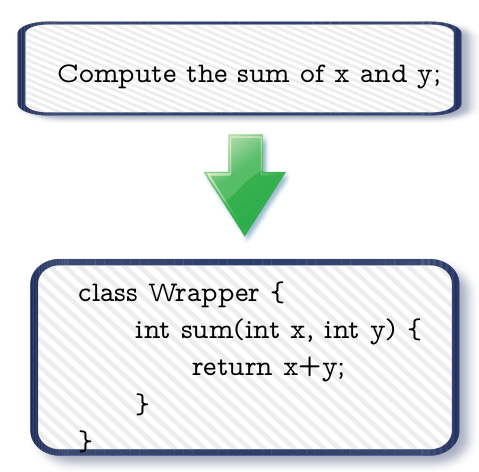
\includegraphics[scale=0.3]{convert.png}
\caption{A simple example of synthsizing the psudo code to its Java implementation}\label{fig:convert}
\end{figure}


\section{Methodology}
We formalize the key idea of our approach through the core language shown in
figure~\ref{fig:language}. 
 
 \begin{figure}
\centering
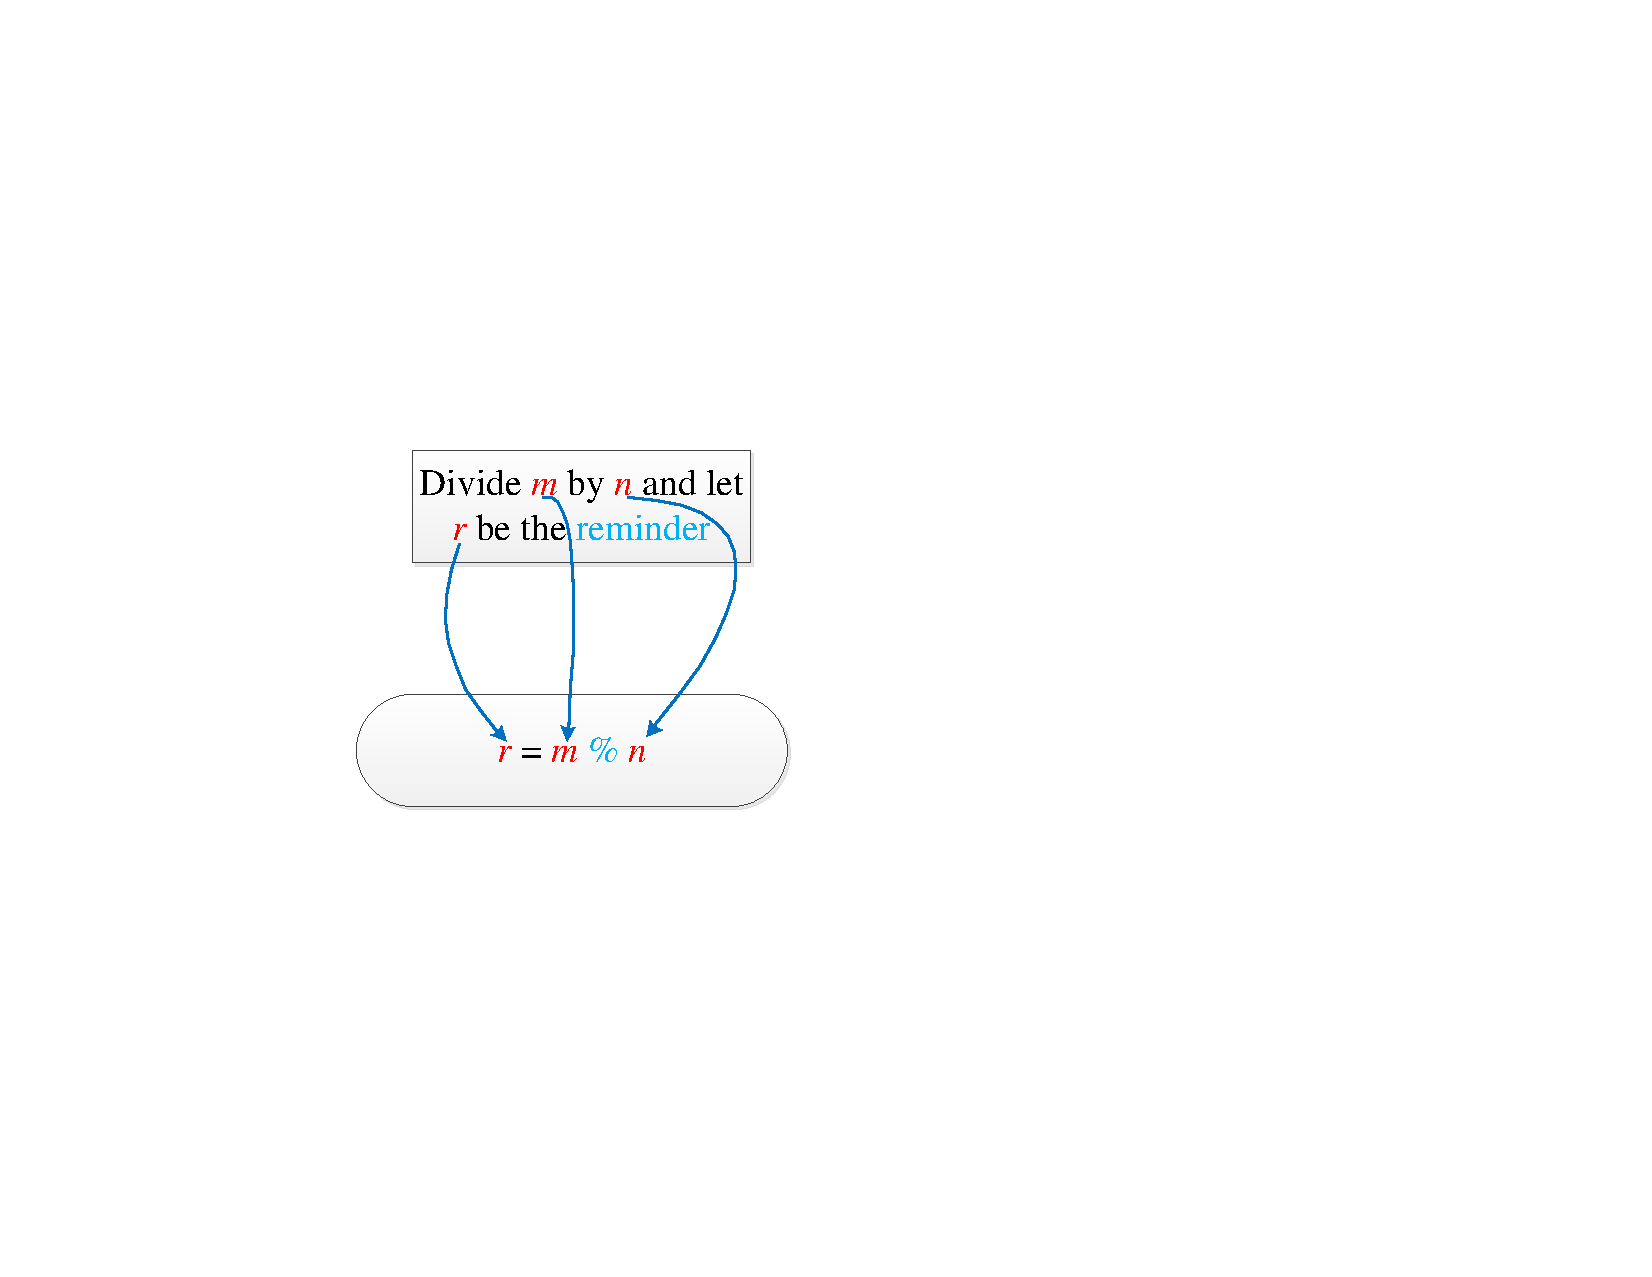
\includegraphics[scale=0.7]{figure2.pdf}
\caption{The first sentence in the euclidean algorithm}\label{fig:align}
\end{figure}

 \begin{figure}[t]
 \small
\[
\begin{array}{lll}
{\rm Program} \ P & := & F^+ \\
{\rm Function} \ F & := &  f(v_1,...,v_i) = S \\
{\rm Constraint} \ C & := & S_1 \uplus ... \uplus S_i \\
{\rm VarDecl} \ V & := & T \  {\rm var\_name}; \\
{\rm Statement} \ S & := & S_1;S_2 | v_1 = v_2 \ | v_1 = v_2 \oplus v_3 \ \\
& & | \ v_1 = v_2.f \ | \ v_1.f = v_2 \\
& & | \ v = {\rm new}^\rho \ T  \ \\
& & |  \ {\rm if}(C) \ I_1 \ {\rm else} \ I_2 \ | while(C) \ do \ S \ \\
& & | \ m^\rho@T(v_1, \ldots, v_n) \ \\
& & | \ v_0.m^\rho(v_1, \ldots, v_n) \\
{\rm Control flow} \ P & := & S_1 \leadsto S_2 \\
{\rm Data flow} \ P & := & v_i \leadsto a_i \\

\end{array}
\]
\vspace{-0.2in}
\caption{Core language used for our formalization. $\oplus$ denotes 
binary operations(+/-/*/\%) and $\uplus$ denotes logical 
operations($<$,$>$,$==$, $\land$ and $\lor$). }\label{fig:language}
\vspace{-0.1in}
\end{figure}
To train a semantic parser so as to map the natural pseudo descriptions into our 
formal intermediate language shown in figure~\ref{fig:language}. 
Our system adopts a template-based approach similar to~\cite{word}. Specifically,  
it models the statements in Figure~\ref{fig:language} as a set of templates
and the problem is reduced to selecting the right templates and alignment. In figure~\ref{fig:align},
 the upper part shows the first sentence of the euclidean algorithm and its lower part
 shows its corresponding template as well as the alignment we need to infer.
Natural language is ambiguous, thus for each set of pseudo descriptions
in an algorithm $x$, there are multiple derivations $i\in I$. Using a 
log-linear model, the probability of a specific derivation $i$ given 
a pseudo description $x$ can be defined as:
\[
  p(i|x;\theta) = \frac{e^{\theta \times \phi(x,i)}}{\sum_{i'\in I}{e^{\theta \times \phi(x,i')}}}
\]
where $\theta$ is the parameter vector of the feature function.  To inference
the correct formal language during test phase, it requires finding the 
most likely derivation $a$: 
\[
f(x) = arg \ max_{a} p(a|x;\theta)
\]
\section{Evaluation and Metrics}

\subsection{Dataset}

Our dataset comes from the following sources: (1) Traditional algorithms 
from textbooks such as TAOCP~\cite{knuth1998art} and CLRS~\cite{clrs}; (2) Mass algorithms from the internet
 such as Stackoverflow and Wikipedia.  

\subsection{Metrics}
Since there is no exiting tool on synthesizing pseudo descriptions, we don't have other tool to compare with. 
To measure the performance of the system, we can evaluate it based on (1) 
the precision of the semantic parser. More specifically,
we manually write down the correct parse tree in the form of our formal language 
and compute the F-score for the parse tree generated by the system. This gives a partial credit to each outcome.
(2) The correctness of the target program. We can generate the implementation of 
the algorithm and ask other programmers to grade its quality.


% include your own bib file like this:
\bibliographystyle{acl}
\bibliography{report}

\end{document}
